\documentclass[12pt,a4paper]{report}
% ---- packages ----
\usepackage{geometry}
 \geometry{
 a4paper,
 total={210mm,297mm},
 left=20mm,
 right=20mm,
 top=30mm,
 bottom=30mm,
 }

\usepackage[utf8]{inputenc}
\usepackage[cyr]{aeguill}
\usepackage{wrapfig}
\usepackage{graphicx}
\usepackage{color}
\usepackage{amsmath}
\usepackage{amsfonts}
\usepackage{amssymb}
\usepackage{pdfpages}
\usepackage[tight]{shorttoc}
\usepackage{hyperref}
\usepackage{verbatim}
\usepackage[english]{babel}
\usepackage{csquotes}
\usepackage{enumerate}
\usepackage{booktabs}
\usepackage{multirow}
\usepackage[inline]{enumitem}
\usepackage[
backend=biber,
style=numeric-comp,
citestyle=numeric-comp,
sorting=ynt
]{biblatex}
\usepackage{listings}


% ---- setup ----
\newcommand{\be }{\begin{itemize}\maketitle}
\newcommand{\en }{\end{itemize}}

\addbibresource{bibliography/github.bib}
\addbibresource{bibliography/online.bib}
\addbibresource{bibliography/papers.bib}
\addbibresource{bibliography/rfcs.bib}
\addbibresource{bibliography/wikipedia.bib}

% section numbering up to subsubsection incl.
\setcounter{secnumdepth}{3}

% list in toc up to subsection incl.
\setcounter{tocdepth}{2}

\setlength{\parskip}{1em}

\begin{document}
\renewcommand{\bibname}{References}
\renewcommand{\chaptername}{Section}

% ---- title page ---
\begin{titlepage}

\newcommand{\HRule}{\rule{\linewidth}{0.5mm}}
\center
 
% headings
\textsc{\LARGE Mickaël Misbach Master Thesis}\\[0.5cm]
%\textsc{\LARGE The Hyve}\\[1cm]

\textsc{\Large École Polytechnique Fédérale de Lausanne \& The Hyve}\\[0.5cm] 
\textsc{\large \reportTitle}\\[0.5cm]

% title
\HRule \\[0.4cm]
{ \huge \bfseries Building a common and privacy-preserving front end for open-source clinical research platforms}\\[0.4cm]
%{ \huge \bfseries \reportTitle}\\[0.4cm]
\HRule \\[1cm]
 
% authors
\begin{minipage}{0.4\textwidth}
\begin{flushleft} \large
\emph{Master Student:}\\
Mickaël \textsc{Misbach}$^{*\dagger}$\\
\end{flushleft}
\end{minipage}
~
\begin{minipage}{0.4\textwidth}
\begin{flushright} \large
\emph{The Hyve Supervisors:} \\
Ward \textsc{Weistra}$^*$\\
Dr. Bo \textsc{Gao}$^*$\\[\baselineskip]
\emph{EPFL Supervisors:} \\
Jean-Louis \textsc{Raisaro}$^\dagger$\\
Dr. Juan \textsc{Troncoso-Pastoriza}$^\dagger$\\[\baselineskip]
\emph{EPFL Professor:} \\
Prof. Jean-Pierre \textsc{Hubaux}$^\dagger$\\
\end{flushright}
\end{minipage}\\[1.5cm]


% logos

\includegraphics[width=0.6\linewidth]{./figures/epfl_logo.png}\\

\includegraphics[width=0.66\linewidth]{./figures/thehyve_logo.pdf}\\

% todo: remove the chapter num from the chapte pages?
% todo: tag repo milestone/1, etc. (and place produced bin)
% todo: have internal cover page for all infos (only titles and logos on first)
% todo: use phd template ? https://phd.epfl.ch/page-149270.html
% todo: make look nicer
% todo: add emails as *{firstname}@thehyve.nl ; +{firstname.lastname}@epfl.ch
% todo: The student must write a report that contains the following items:
% The title
% The student’s contact details (surname, first name, address)
% The name of the IC laboratory, the name of the company or the name of the other university in
%which the master thesis is being done
% The name of the responsible IC professor
% The results of the thesis (analysis, conception and implementation)
%The report must be representative of the student’s work in order to be able to judge the student’s ability
%to be an engineer. The project will be archived within the sections and, in general, in the laboratory of the
%IC professor. The report must not contain any confidential information, except in exceptional cases. 

\vfill

\end{titlepage}


% ---- abstract ----
\newpage
\newgeometry{left=3cm,right=3cm}
\begin{abstract}

% problem / motivation
Being able to exploit large and heterogeneous medical data is crucial for realizing the promise of precision medicine to its full potential. 
Yet, currently, due to the presence of multiple and fragmented systems at different clinical sites, it is often difficult to enable researchers to access the data they need. 
Privacy and security concerns also represent major obstacles that need to be overcome in order to provide access to sensitive medical data that are usually not exposed by clinical sites for the fear of data leaks. 

% solution / key idea
To address these challenges, we propose a system that employs Glowing Bear as a common front end to the widespread clinical research platforms i2b2, tranSMART and MedCo.
Our proposed system uses IRCT, the official implementation of the PIC-SURE API, which acts as an interoperability layer that translates clinical research queries into native API languages.
With our work, we take a step towards the technical convergence of i2b2 and tranSMART, giving clinical sites the means to share their data more easily.
Even more, with the support of MedCo, a cohort explorer with strong privacy and security guarantees based on federated i2b2 instances, we enable clinical sites to share sensitive data that would be difficult to share otherwise.

\end{abstract}
\restoregeometry


% --- table of contents pages ----
\newpage
\tableofcontents

% ---- content ----
\newpage
% todo: have disambiguation if needed
% vocabulary
% query terms: concepts (i2b2) / constraints (more than that) / tree node
% query term type
% query: constraints
% data sources (no pic-sure resource)
% "paper" rather than thesis or document
% ============================

% flow of the paper:
% \begin{itemize}
%     \item motivation exposes problems
%     \item problems to be solved lead to objectives
%     \item objectives translated into technical requirements
%     \item technical requirements met with architecture solution
%     \item solution designed and implemented
%     \item evaluation of how implementation meet requirements
% \end{itemize}

\chapter{Introduction}
% todo: add citation in here
% 1: https://www.karger.com/Article/FullText/481682 : cite

% precision medicine what it needs
Realization of the promise of precision medicine requires large and diversified clinical and genomic data sets for researchers to exploit~\cite{todo1}.
Existing technical solutions to exploit those data sets exist and are widely used, the two main open-source players being i2b2 and tranSMART.

% data scattered in systems
However those clinical research platforms are generally deployed at single clinical sites, or at best a group of them, hosting their own data.
This leads to the presence of multiple and fragmented systems at different locations all over the world, a situation that is not close to change as a lot of effort and money has been invested in those by clinical sites on often tight budgets.
Due to this scattered data, researchers find themselves limited by the amount of data that their own clinical sites produce.

% data sharing
A straightforward solution to this problem is to share the data between the clinical sites, however this faces two challenges.
First challenge is technical, the different clinical research platforms are not interoperable together.
Second is legal and ethic, as medical data are highly sensitive information about individuals.
Those are protected by strict regulations such as HIPAA in the US or GDPR in EU, and data leaks could be devastating to the concerned persons, thus privacy and security guarantees are capital.

% solution to this \ contribution
In this paper we build a system that takes a step towards the technical convergence of those systems by providing an interoperability layer for i2b2 and tranSMART, exploitable by a unique front end, Glowing Bear.
Moreover this interoperability layer offers as well the ability to securely share medical data between clinical sites using the privacy-preserving system MedCo.


\section{Problem Statement}
\label{sec:problem}

\subsection*{Motivation}


% todo: get inspiration from papers
% 2 problems (here)  --> 2 objectives (in objective)

% IMPORTANT: why do these 2 objectives should be taken together, and not separately, and why not others

\subsection*{Objectives}
% check http://www.ceptara.com/blog/how-to-write-problem-statement
%-Why this is a hard/open problem?
%-State-of-the-Art not sufficient (refer to related work?)
% goal: solving this problem: goal: common - privacy preserving

% facilitating adoption / meaningful things -> open-source / docker / secure / etc (overlap with requirements? or should that go to the requirements? check how to split)
% 2 problems (from motivations)  --> 2 objectives (here)


% These characteristics define two main objectives to fulfill. 
% First, the front end in question will need to be able to communicate with the main open-source several clinical research platforms, to cover a major part of the platforms used by researchers.
% Second, the front end , namely MedCo, the only privacy-preserving platform.
% todo: in the analyses of what are the platforms, mention what they are

% --> focus on cohort exploration (why?)


\begin{itemize}
    \item data scattered in several ways / all the constraints that prevent what said previously to be achieved
    \item physically in different institutions / organizations
    \item technologically heterogeneous, (backend systems, apis to access, semantic different, etc.)
    \item legal constraints, risk of leaks
    \item  patients reluctant to share their data
\end{itemize}

% todo: emphasize, bold or italic, the objectives
% 2 obj that stem from Enable scientists to access more data from a common interface by...
\begin{itemize}
    \item common system to unify different system, have a common one
    \item accessing sensitive data that would otherwise not be shared
\end{itemize}

% FROM WARD
% ======== motivation exposes problem


Combining data from these different data warehouses is hard because of technical and interoperability reasons. In this paper we will focus on the first problem. Moving all data to one data warehouse is not feasible, because of the amount of work to do so and because different data warehouses are specialized in different data types (structured clinical data, large scale genomics data, etc.).

Also, although there are many different data warehouses for health care data, many of them need similar functionality: patient cohort selection, data selection, exploratory analysis, export functionality. However, different data warehouses currently waste financial and development resources on building and maintaining their user interfaces.

% ======== problems solved to objectives 
In this paper we aim to:
- allow one existing, modern data warehouse user interface, with an interoperability layer, to run on multiple data warehouses, specifically the i2b2, tranSMART and medco data warehouses.
- lay the basis for allowing multiple specialized data sources to connect to one user interface, allowing the user to combine information from patients spread over them.


\section{Solution Requirements}
\label{sec:requirements}

% requirements list
We translate the objectives stated in~\ref{sec:problem} into the following requirements.
Our solution must:

\begin{enumerate}
    % the systems ARE a requirement
    \item be compatible with the two major open-source clinical research systems: tranSMART (v17.1) and i2b2  % todo: and do what exactly? cohort exploraiton blabla, goal is not just to be compatible
    \item enable sharing of sensitive data in a privacy-preserving way: with MedCo
    \item be free of technical constraint against its use, by:
    \begin{enumerate}
        \item being easy to deploy, even in existing environments
        \item not degrading the experience of existing systems
        \item being secure
        \item being open-source
        \item having a practical runtime
        \item being future-proof
    \end{enumerate}
\end{enumerate}

% why requirements are fulfilling objectives

% reasons for open-source:
% In the open-source spirit, existing technologies and standard. Maximizing the value of the work. 
% Integrating with existing systems.

from ward:
% ======== objectives into technical requirements
Interoperability layer
Medco, tranSMART, i2b2
Support for multiple data sources (in the basis)

\section{Solution Overview}

\begin{itemize}
    \item big picture of the whole system in short
    \item how it helps solve the 2 objectives in short
\end{itemize}


\section{Contributions}

\begin{itemize}
    \item list of contributions made
    \item evaluation shows how the contributions are successful
\end{itemize}

% - what we do is a step in the direction of blabla
% convergence of blabla

\section{Outline}
TBD

\chapter{Background \& Related Work}
\label{sec:bg-relwork}

\section{Background}
This section offers some important background information providing context to what is presented in the later sections. 

\subsection{i2b2}
\label{sec:bg-i2b2}

% features
I2b2 is a clinical research platform used for cohort exploration.
The server is written in Java and using Apache Axis2~\cite{todo} for its web services, it exposes an XML API to interact with it.
Its source code is organized by \emph{cells} in a \emph{hive}.
The \emph{CRC} (Clinical Research Chart) cell is the data repository containing the patients data, the \emph{PM} (Project Management) cell contains all information about users and metadata about the data in the CRC, the \emph{ONT} (Ontology) contains the ontology with which the data is structured.

% db
It stores patients data in this relational database encoded in a star schema.
This schema has a central table \emph{observation fact} that records any kind of observation about a patient.
This table stores a unique set of references to its satellite dimension tables, each containing information about the \emph{patient}, the \emph{ontology concept} observed, the \emph{encounter} that led to the observation and the \emph{provider} that did it.
The data is structured around standard ontologies such as \emph{ICD9}~\cite{todo}.

% client
I2b2 has two official clients.
First the \emph{webclient} is a Javascript application running is web browsers and built around the \emph{yui}~\cite{todo} framework.
Second is the \emph{workbench}, a Java desktop application doing the same thing and a bit more.
Both communicate with the server with the i2b2 XML API.

\subsection{tranSMART}

% features
TranSMART is also a clinical research platform, offering cohort exploration but also more advanced analysis on these features.
It is written mostly in Groovy~\cite{todo}, which runs in the Java Virtual Machine, and offers a modern JSON API in its latest version 17.1.

% db
The core data schema is the same as i2b2 with two additional dimension tables: \emph{studies} which represent a medical study from which data has been obtained, and \emph{trial visits} recording progression through time of a study.
Its data is structured around the \emph{studies}, which each have their own ontologies.
Some ontology concepts can be shared among studies and can be used as \emph{cross-study concepts}.

% client
Its official client is a web application rendered in Java on the server-side called \emph{tranSMARTApp}.


\subsection{PIC-SURE API}
\label{sec:bg-picsure}

% intro
The PIC-SURE (Patient-centered Information Commons: Standardized Unification of Research Elements)~\cite{PIC-SURE} API is a generic API with a SQL-like syntax that aims to query different patients-centered data warehouses.

% resource, clauses
PIC-SURE is \emph{resource}-based: each data source (e.g. i2b2) is considered a resource.
To query these resources, the user of the API uses \emph{clauses} submitted to the API \emph{Query Service}.
Four types of clauses are supported: \emph{select}, \emph{where}, \emph{process} and \emph{join}.
Here we focus only on \emph{where} clauses, which are the only ones used with i2b2.

% where 
The \emph{where} clause is used to specified constraints on the queried data.
The resource declares the \emph{predicates} that its \emph{where} clauses support.
To give input to the predicates, the predicates declare \emph{fields}.
Each of those fields take a value as input, whose type is declared.
Example of a \emph{where clause}:
\begin{verbatim}
"where": [ {
    "field": {
        "pui": "/resource/study/Age/",
        "dataType": "INTEGER"
    },
    "predicate": "CONSTRAIN_VALUE",
    "fields": {
        "OPERATOR": "GT",
        "CONSTRAINT": "20"
    }
} ]
\end{verbatim}

% tree
In order to construct queries, the resources expose a tree of query terms uniquely identified by a path, through the API \emph{Resource Service}.
Each of those query terms, if they are queryable, declare a data type.
Each of the predicates used for the \emph{where} clauses also declare one or more supported data types: this is the mechanism used to know which query terms support which predicates.
In order to link the tree nodes together, the resources declare what kind of relationships between nodes exist.
For example if the tree supports the relationship \verb|CHILD|, a client can request all the children of a certain node. 


\subsubsection*{IRCT}

The official implementation of the PIC-SURE API is called Inter Resource Communication Tool (IRCT), and is the combination of four different components that are open-source and available on~\cite{IRCT-github}. 
They are implemented in Java and use standard technologies: web application archive (WAR)~\cite{wiki:war} for deployment, Hibernate~\cite{wiki:hibernate} for data storage.
First the Communication Layer (IRCT-CL) implements the RESTful PIC-SURE API. 
The core component is the Application Programming Interface (IRCT-API), it handles the execution of queries and processing of results.
An instance can be extended using the IRCT Extension (IRCT-EXT) that provides hooks and additional features without having to modify the core code.
Finally the Resource Interface (IRCT-RI) connects to the different resources through connectors.
Resources are registered and defined in the database.
Their definition include all the predicates, operations, relationships, etc. they support.


\subsection{Glowing Bear}

% intro & features
Glowing Bear is a front end web application built using Angular as an new user interface to tranSMART 17.1.
Angular is a Typescript~\cite{todo} framework to develop web applications.
Typescript is a language that when compiled produce javascript code to be run inside a web browser.
Glowing Bear offer basic cohort exploration features, but also advanced analytic features or data export.

% services, components
Its source code is organized in mainly Angular services and components.
Services are singleton objects that handle logic related to data.
Among others the notable services in Glowing Bear are the \emph{Tree Node Service}, handling data relate to the tree of query terms or the \emph{Resource Service}, handling communication with the back end.
Components contain the logic of representing the data, and associate an object that contain the component logic, and a HTML template that displays it.


\subsection{OpenID Connect}

% todo: claim, jwt
% todo: backgorund about oidc (client id, etc.)
% todo: list of requirements from the standards


OpenID Connect is a protocol enabling authentication and authorization using a third-party implementing the server-side of the protocol.
It offers several types of negotiations (called \emph{flow}) between the server and client(s), but they all end up with an access token used by a user to access a resource.
This token is standardized as a JSON Web Token (JWT)~\cite{todo}.

\subsubsection*{JSON Web Token}
% todo: cite rsa paper and sha and jwt and oidc

A JWT is three distinct base64-encoded values separated by a dot: two JSON objects and a signature.
The first is the header, which contains metadata about the JWT, such as the signing algorithm used and the identifier of the key used to perform the signing.
Example:

\begin{samepage}
\begin{verbatim}
{
  "alg": "RS256",
  "typ": "JWT",
  "kid": "eTFrdyrNxXLNHI7p0Ywybc7z1SBHTEcqWcMTybtdvQY"
}
\end{verbatim}
\end{samepage}

The second is the payload of the JWT, and contains the identity of the authenticated user, its authorizations, and can contain any kind of custom fields set up by the administrator of the OIDC server.
Other standard fields include expiration time, client identifier, token issuer, etc.
Those data are called the JWT claims.
Example:


\begin{verbatim}
{
  "jti": "6fd4f480-05ce-471f-a4ef-f35cb6a8e0d0",
  "exp": 1523454086,
  "nbf": 0,
  "iat": 1523453186,
  "iss": "http://localhost:8081/auth/realms/master",
  "aud": "glowing-bear",
  "sub": "df110f80-fa32-4174-970d-e42a7b24ae9f",
  "typ": "Bearer",
  "azp": "glowing-bear",
  "nonce": "N0.28573339803406971523453198656",
  "auth_time": 1523453186,
  "session_state": "74cd6393-9d24-4140-a87a-9e557f45499b",
  "acr": "1",
  "resource_access": {
    "account": {
      "roles": [
        "role1",
        "role2"
      ]
    }
  },
  "preferred_username": "test",
  "email": "test@test.com"
}
\end{verbatim}

The last value is a signature generated by the OIDC server that serves two purposes: verify that the issuer was indeed the OIDC server, and protect the integrity of the token.
Several algorithm can be used to generate this signature, here we use the algorithm \emph{RS256}, i.e. the encryption of a \emph{SHA256} hash using the asymmetric cryptosystem RSA.


\subsection{MedCo}
\label{sec:bg-medco}

MedCo is a system of federated clinical sites sharing data together in a secure and privacy-preserving way.
Its security relies on a collective authority~\cite{todo} formed by all the MedCo nodes.
It uses an homomorphic cryptosystem, which means that some operation on encrypted data is possible. 
Each of the node has a public and private key, and by assembling all the public keys together the public key of the collective authority is generated.
The corresponding private does not exist, thus all operations requiring the private keys are distributed across all nodes using specific protocols.

For more detailed information about MedCo and its underlying technologies, please refer to~\cite{todo}.

\section{Related Work}

Our literature review focus on approaches similar to our main contribution, an interoperability layer for clinical research systems coupled with a front end.


\paragraph{SHRINE}

SHRINE (Shared Health Research Informatics NEtwork)~\cite{shrine} is a system that allows to network i2b2 instances together.
From a single webclient, a fork of the i2b2 webclient, several i2b2 can be queried at the same time, and their results be displayed in a unique interface.
By this, SHRINE offers an interoperability layer over an arbitrary number of i2b2 instances.
SHRINE's design is very tightly linked to i2b2 and extending its support to additional clinical research system is not possible.


\paragraph{Borderline}

% borderline
\emph{Borderline}~\cite{borderline} is a set of services that includes a user interface, and several back end components.
The user interface allows users to query clinical research platforms.
This UI communicates with its back end which manages the queries and proxies them to the connectors.
The connectors are responsible to query platforms containing patient data, such as tranSMART.
Borderline is a more of a query workflow management tool rather than a proper cohort explorer, and it is at the time of writing still a work-in-progress.



% check citations from other papers (bd2k and others)

% other systems:
% borderline:
% https://github.com/dsi-icl/borderline-server
% https://github.com/dsi-icl/borderline-middleware
% Etriks Analytics Environment
% https://eae.etriks.org/eae/


% - https://academic.oup.com/jamia/article/22/6/1132/2357622?searchresult=1
% - https://github.com/hms-dbmi/hackathon-Sept2017
% - http://dbmi.hms.harvard.edu/news/datathon-hackathon-sep-14-15
% - http://orthuber.com/MIE2009p0584.pdf
% - https://en.wikipedia.org/wiki/MultiDimensional_eXpressions
% - http://journals.sagepub.com/doi/abs/10.1177/1473871614526077
% - https://academic.oup.com/jamia/article/22/6/1114/2358127
% - https://www.nature.com/articles/sdata201696.pdf
% - https://www.sciencedirect.com/science/article/pii/S1532046417300709
% - 
% - CAVA: http://perer.org/papers/adamPerer-CAVA-IVS2014.pdf
% - http://orthuber.com/MIE2009p0584.pdf
% - explore refs of i2b2/shrine papers
% - is there transmart paper?
% - http://journals.sagepub.com/doi/abs/10.1177/1473871614526077: stopped at 18
% how to write: 
% - http://wiki.openi.org/openi-plug-in-for-i2b2

% todo: mention data sharing initiatives? all of us, eu initiatives


%they had a partnership with pic sure: %https://academic.oup.com/jamia/article/22/6/1132/2357622?searchresult=1
%pic sure 'wow' story (nhanes): %https://bd2kccc.org/wp-content/uploads/2017/02/15_PIC-SURE_FInal.pdf


\chapter{System Architecture}
\label{sec:sysarchitecture}

To design a system fulfilling the requirements listed in \ref{sec:requirements}, we start from the bottom by first choosing its basic building blocks, and then we explore the different ways in which they can be assembled.
Finally we show an overview of the final system.
By the requirements, we only consider open-source technologies.


\section{Choice of Open-Source Technologies}

% outline
The choice of the open-source technologies to use depends mainly on the clinical research platforms that we aim to support.
First we review those platforms, then we explore existing open-source front end systems in hope of determining if one of them is worth being used for our solution.
Finally we motivate the delegation of identity and access management to an identity provider, and choose a software that implements it.

\subsection{Back End Systems: Clinical Research Platforms}

% what is a clinical research platform
A clinical research platform is a back end software (i.e. running on server, serving request to clients), that stores any kind of medical data and can answer queries, with the purpose of identifying patient cohorts, and possibly performing analysis on those data.

% use-case 
Queries on this data can be for any purpose, here follows two example use-cases for this kind of platform.
\begin{itemize}
    \item An oncologist at an hospital tries to identify response to specific medications according to criterion such as the presence of some alleles in the genome of the patients.
    \item A pharmaceutical company wishes to conduct a study on a new medication, and needs to recruit a cohort of young patients that had a specific diagnoses at some point in time.
\end{itemize}

% use-case: technical
We cover in this document the basic technical requirement of these use-cases: obtaining patient counts based on inclusion and exclusion criterion.
Of course more processing can be done, such as statistical analysis, but this is not the focus here.

% i2b2 / transmart: they do the above, and allow this use-case, star schema
The two main players in terms of open source clinical research platforms are \emph{i2b2}~\cite{todo} and \emph{tranSMART}~\cite{todo}.
They enable the use-cases presented before by leveraging on an almost identical database schema: the star schema. 
This schema has a central table containing \emph{observation facts}, and several dimension tables: \emph{patient}, \emph{visit}, \emph{concept} and \emph{modifier}.
And specifically for tranSMART: \emph{study} and \emph{trial visit}.
An observation is a dated record of an event that refers to entries in the aforementioned dimensions.
We choose to support these two platforms, in their latest version at the time of the project, as together they host an enormous amount of data hosted by hospitals, research institutes or pharmaceutical companies.

% medco
MedCo~\cite{todo} is a privacy-preserving clinical research platform, and at the time of the project the only one that offers privacy-preserving guarantees.
It enables the sharing of sensitive medical data within a federated group of clinical sites in a privacy-preserving way by using homomorphic encryption and obfuscation techniques.
MedCo fits our requirements and use-cases as it is open-source, based on i2b2, and allow count queries based on inclusion and exclusion criterion, with end-to-end encryption.


\subsection{Front End System: Cohort Explorers}

% requirements for front end
To build our front end we have several systems on which we could base our solution on.
We require it to be modern, open-source, web-based for portability, and if possible at least partially compatible with the clinical research platforms we support.
If all those requirements can not be met, there is left the option of building the front-end from scratch, but as seen in this section we manage avoid this significant effort.

% list of candidates
The result of a review of available open-source front-end for cohort exploration who deserve to be investigated follows:
\begin{itemize}
    \item i2b2 webclient~\cite{todo}
    \item i2b2 workbench~\cite{todo}
    \item transmartApp~\cite{todo}
    \item Glowing Bear~\cite{todo}
\end{itemize}

% i2b2 webclient / workbench and transmartapp
Each of the previously retained platforms have their official web front end: the \emph{i2b2 webclient} for i2b2, and \emph{tranSMARTApp} for tranSMART.
Both of them are perfectly compatible with their respective back ends, however they suffer from two major problems:
\begin{enumerate*}
    \item they use old or outdated technologies, making future development and maintenance more difficult;
    \item they are very tightly linked to their back end, making the development of support for the other difficult.
\end{enumerate*}
The \emph{i2b2 webclient} uses \emph{yui}~\cite{todo}, a javascript framework developed by Yahoo, and not supported anymore since 2014. 
\emph{tranSMARTApp} is a web application rendered on the server-side in Java, alongside tranSMART, and not a pure web client.
For those reasons we choose to not retain those solutions.
We can also mention the \emph{i2b2 workbench}, client desktop application for i2b2, but as it is not web-based we discard it as well

% introduce gb yep
\emph{Glowing Bear} is the front end system we choose to retain.
It is modern, web-based and mature software. 
It is implemented on top of tranSMART (v17.1) but its source is structured generically, facilitating the implementation of support for other platforms.
It thus fits all of our requirements for a front end.


\subsection{Identity Provider}

Such a system with different components calls for a common and standardized way of handling authentication and authorization.
The de-facto modern standard for this is the OpenID Connect protocol~\cite{todo} (OIDC), which we are using in our solution.
OIDC allows to externalize in a secure way authentication and authorization in a multi-components system.
A stable, mature and open-source implementation of OIDC is the server software Keycloak~\cite{todo}, that we choose to use.


\section{Building the System Architecture}

\subsection{Assembling the Building Blocks}

% intro
Now that we have the basic building blocks of our solution, we design a system where they fit together in a coherent way.
The architecture can roughly be categorized in three zones:
\begin{itemize}
    \item Front end
    \item Interoperability layer
    \item Clinical research platforms
\end{itemize}
Our building blocks lies in the front end and clinical research platforms zones. 
We now are designing the interoperability layer that connects those two zones.

% assembling
This interoperability layer can be implemented in the front end, in the back end or in both.
Because the front end Glowing Bear implements the compatibility with tranSMART, we could imagine that implementing the interoperability layer into Glowing Bear by adding the support for i2b2 and MedCo, using the i2b2 XML API, alongside tranSMART.

% front end
However for two reasons we want to avoid a fully front end i2b2 API implementation: 
\begin{enumerate*}
    \item the i2b2 XML API is old and cluttered, which means difficult to implement and maintain;
    \item by only implementing the support for specific systems, this would not leave much space for extensibility.
\end{enumerate*}

% back end
\begin{samepage}
Second option is implementing the layer fully in the back end, which would mean that:
\begin{itemize}
    \item we need a back end component to take care of the APIs translation
    \item the support of tranSMART in Glowing Bear would be removed and re-implemented in the back end component
\end{itemize}
While the first consequence is not a problem, the second implies pretty heavy additional work, with not much added value.
\end{samepage}


% we choose both
For the reasons enumerated before, we choose in our system the hybrid approach: implementing the interoperability layer in both the front end and the back end.
In the front end the support of tranSMART is kept, and we use a back end component to take care of the translation to the other clinical research platforms, i2b2 and MedCo, all the while having Glowing Bear communicating with this component with a unique API.

% pic-sure
For this task the \emph{PIC-SURE} API~\cite{todo} is the perfect tool.
It is a generic API that was designed to be translated to any kind of API used for querying medical data, and supports several systems, including i2b2.
The back end component implementing the PIC-SURE API is \emph{IRCT} and is open-source.
Thanks to its extensibility capabilities, we are using as well to implement support for MedCo.
Support for the additional systems that IRCT is compatible with is left for future work.

% ccl
To summarize, our interoperability layer is composed of 
\begin{enumerate}
    \item an interoperability module in  Glowing Bear, which has support for both the tranSMART REST API v2, and PIC-SURE;
    \item IRCT, which has support for i2b2 and MedCo.
\end{enumerate} 

\subsection{Technical Choices Summary}

We summarize our technical choices:

\begin{itemize}
    \setlength\itemsep{0em}
    \item Supported clinical research platforms: \emph{i2b2 1.7}, \emph{tranSMART 17.1}, \emph{MedCo}
    \item Interoperability layer for i2b2 and MedCo: \emph{IRCT} (PIC-SURE API)
    \item Front end with support for tranSMART REST API v2 and PIC-SURE: \emph{Glowing Bear}
\end{itemize}


\begin{samepage}
\subsubsection*{Technical Considerations}

Additionally we take into consideration some software engineering considerations, which allows us to meet or alleviate the technical constraints listed in the requirements.
\begin{enumerate}
    \item A practical query run time: the overhead of using our solution compared to the original clinical research platforms should be negligible.
    \item Extensible: building support for additional systems should be made easy.
    \item Preserve existing user experience: the existing technologies that are used should not be modified in a way that degrades existing features.
    \item Using standards: use existing standard APIs and technologies to the best extent possible.
    \item Quality: produce quality code to facilitate maintenance and encourage reuse
\end{enumerate}
\end{samepage}


\subsection{System Overview}
\begin{figure}[ht]
    \centering
    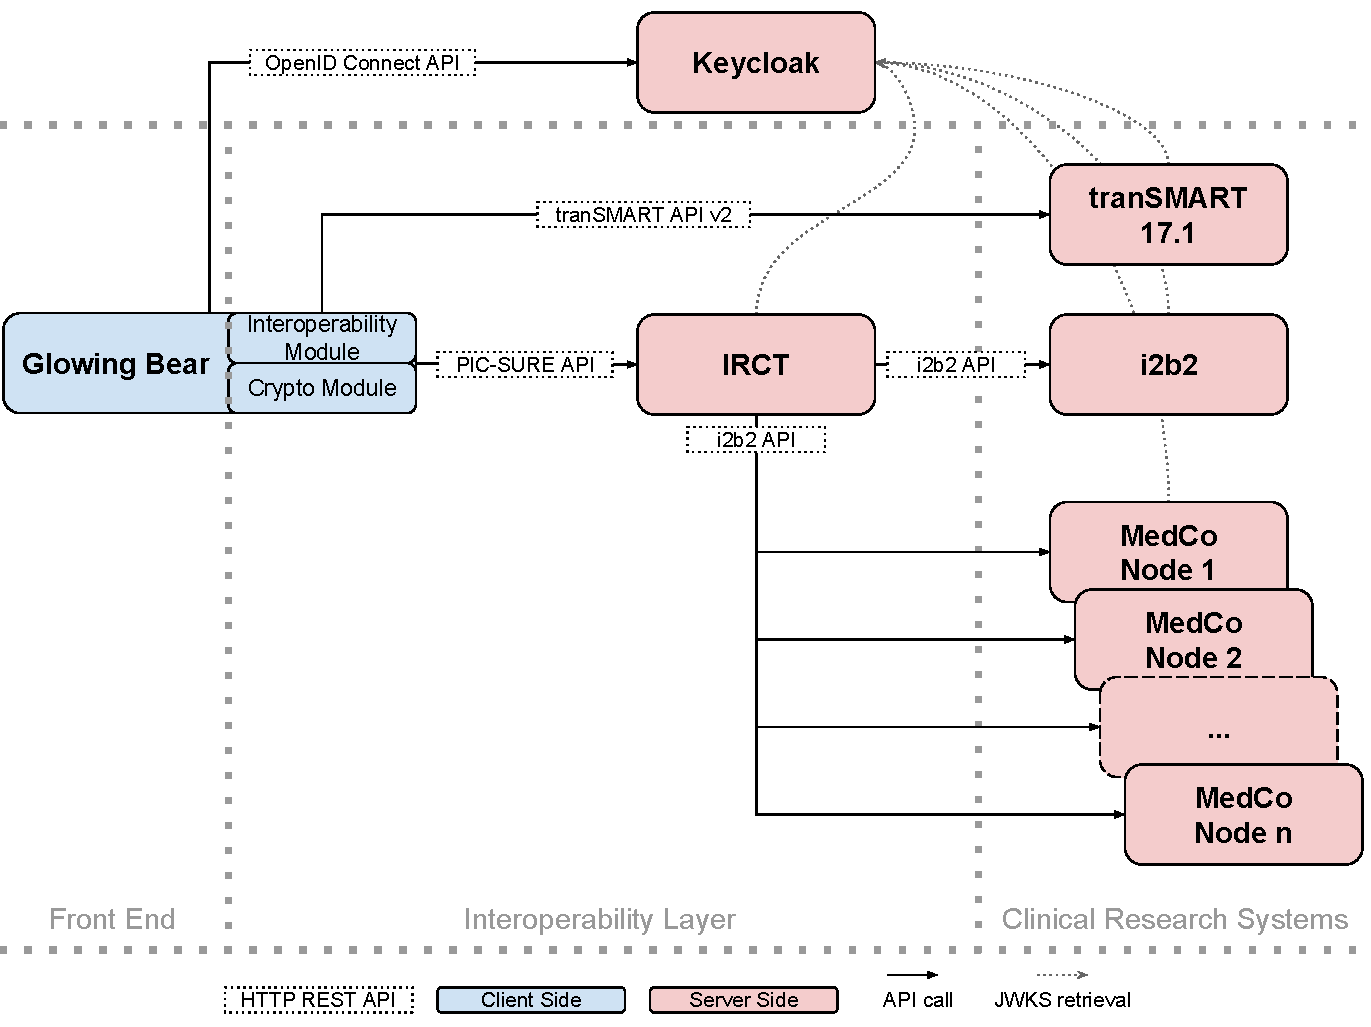
\includegraphics[width=1\textwidth]{figures/sys_diagram_full.pdf}
    \caption{Full System Diagram}
    \label{fig:sys-diagram-full}
\end{figure}

Figure~\ref{fig:sys-diagram-full} shows the architecture of our solution as described in this section.
The high-level idea of the workflow is the following:
\begin{enumerate}
    \item \label{enum:wf-init} While loading Glowing Bear, the user logs in with Keycloak.
    \item The user constructs a query, and Glowing Bear submits it through the appropriate channel:
    \begin{enumerate}
        \item \label{enum:wf-transmart} \emph{tranSMART}: from Glowing Bear, the query is immediately submitted to tranSMART.
        \item \label{enum:wf-i2b2} \emph{i2b2}: from Glowing Bear, the query is submitted to IRCT using the PIC-SURE API, and IRCT submits to i2b2 the query
        \item \label{enum:wf-medco} \emph{MedCo}: using the cryptographic module in Glowing Bear, the query is submitted to IRCT and then broadcasted to all of the MedCo nodes.
    \end{enumerate}
    \item \label{enum:wf-results} The result is fetched and displayed to the user in Glowing Bear. In the case of MedCo the cryptographic module is used to decrypt the result.
\end{enumerate}

The design of step~\ref{enum:wf-init} is covered in section~\ref{sec:interoplayer-idp}, 
step~\ref{enum:wf-i2b2} in section~\ref{sec:interoplayer-gb} and~\ref{sec:interoplayer-picsure}, 
step~\ref{enum:wf-medco} in section~\ref{sec:medco} and finally 
step~\ref{enum:wf-results} in section~\ref{sec:interoplayer-gb}.
Step~\ref{enum:wf-transmart} is not covered in this document as the support for tranSMART in Glowing Bear is preexisting.


\chapter{Interoperability Layer for Clinical Research Systems}
\label{sec:interoplayer}

% intro
Now that we have the architecture of our solution, this chapter covers the design and implementation of the first objective of our project: creating an interoperability layer for the clinical research systems i2b2 and tranSMART 17.1, that is exploitable by the front end Glowing Bear, and with the identity and access management handled by Keycloak.
Support for MedCo is covered in the next section.

% outline
We are first going over the detailed workflow of the system, showing the end-to-end processing of a query.
We are then detailing the design and implementation of the different parts solving the objective: the identity provider, the front-end, the API translation, and the processing in the back end systems.
Appendix~\ref{sec:docker} covers exhaustively the technical details of the Docker-based deployment of the system.


\section{Detailed Workflow}
\label{sec:interoplayer-wf}

\begin{figure}[ht]
    \centering
    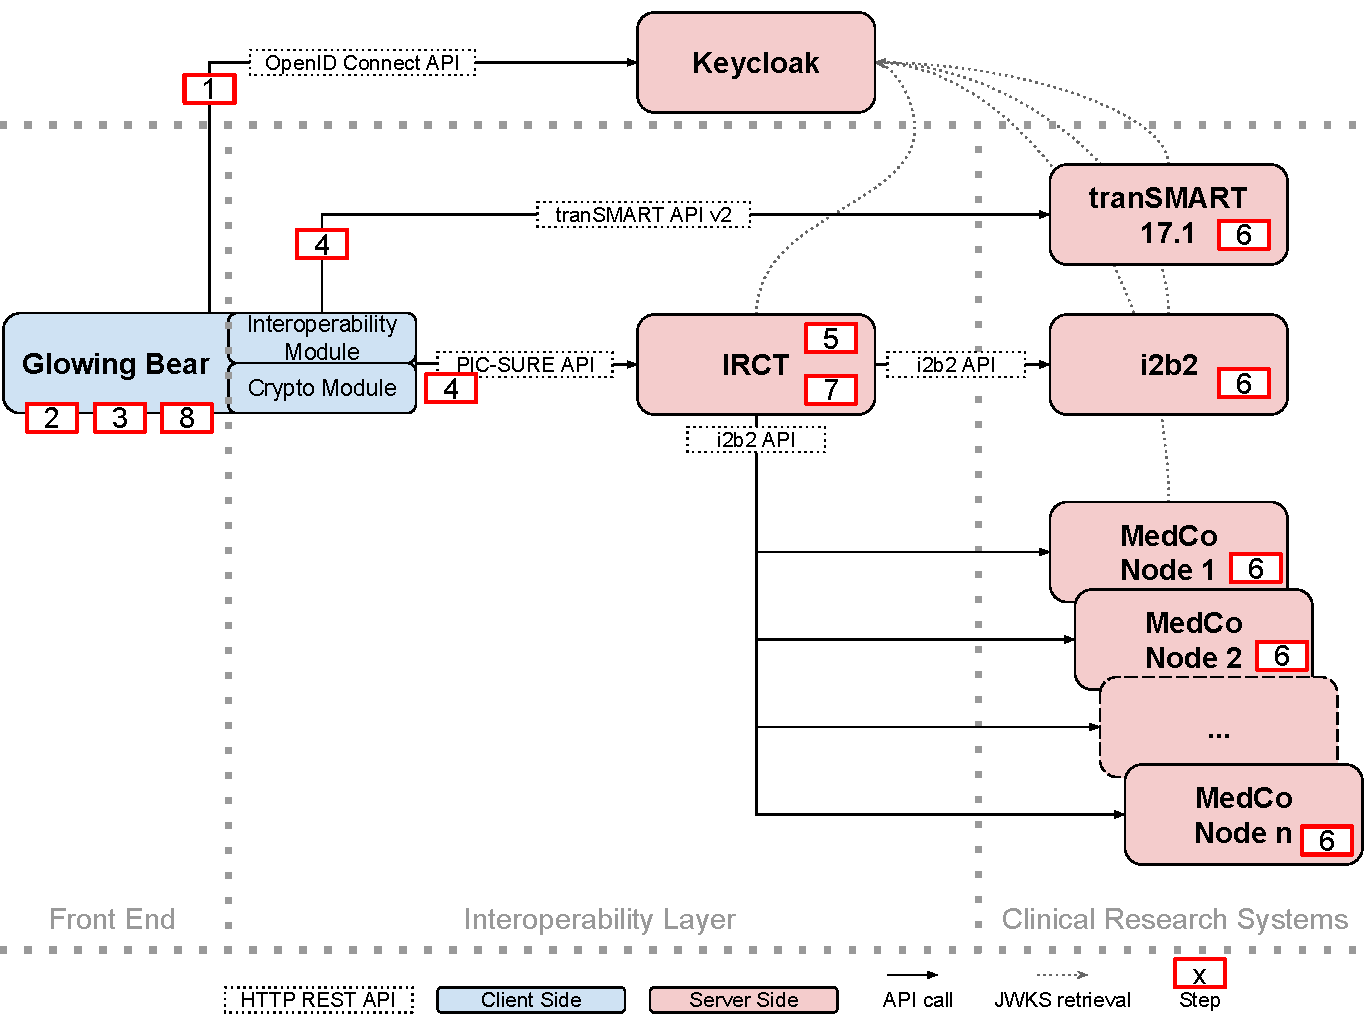
\includegraphics[width=1\textwidth]{figures/sys_diagram_full_with_steps.pdf}
    \caption{Full System Diagram, with execution steps}
    \label{fig:sys-diagram-full-steps}
\end{figure}

This section gives an overview of the full workflow of our system when constructing and executing a query.
Some steps are specific to \textit{tranSMART} 17.1 or \textit{PIC-SURE}.
The step numbering refers to figure~\ref{fig:sys-diagram-full-steps}.

\begin{enumerate}
\item \label{enum:wf-interop-login}\textbf{User Login}:
The user accesses Glowing Bear through its web browser, which redirects it to the Keycloak login page.
The user submits her credentials to Keycloak, which upon success redirects the user to Glowing Bear, giving at the same time the JSON Web Token (JWT)~\cite{rfc:jwt}, containing authentication and authorization information.
The user is thus logged in in the system.

\item \label{enum:wf-interop-init} \textbf{Glowing Bear Initialization}:
Glowing Bear reads from its configuration which type of back end it should use.
The tree of query terms is loaded, either entirely (\textit{tranSMART}) or only the root nodes (\textit{PIC-SURE}).
In the \textit{PIC-SURE} case, Glowing Bear fetches the definitions of the data sources set up on IRCT.

\item \textbf{Query Construction}:
The user browses the tree of query terms and uses them to construct a query corresponding to a patient set.
When adding a term into the query panel, Glowing Bear might, according to its type, make a background request to fetch the term metadata, which is the case for example for categorical or numerical terms.
The user then optionally sets value(s) to the query term.

\item \textbf{Query Submission}:
Upon user request (or automatically according to the configuration), Glowing Bear submits the query to the back end.

\item \textbf{Query Translation} \textit{PIC-SURE only}: IRCT uses the appropriate data source interface to perform the translation into the native i2b2 API of the query, and submits it to i2b2.

\item \textbf{Query Processing}: the submitted query, either directly from Glowing Bear for tranSMART or through IRCT for i2b2, is processed by the platform. 
The result is sent back to the requester.

\item \textbf{Result Storage} \textit{PIC-SURE only}: IRCT stores the result in its database, and sets the query as being successful.

\item \textbf{Result Display}: the result is displayed to the user in Glowing Bear.
Given the asynchronous nature of IRCT when processing queries, Glowing Bear periodically (every second) fetches the status of a \textit{PIC-SURE} query, and only after fetches its result.

\end{enumerate}


\section{Identity and Access Management}
\label{sec:interoplayer-idp}

% outline
This section first exposes how the authentication (identity) and authorization (access) are handled in our system with OpenID Connect and Keycloak, and then the steps taken to achieve this implementation.

\subsection{Authentication}

% overview
Authentication management is about verifying the identity of the user trying to access data.
With OpenID Connect, the authentication of the user is made by the identity provider, here Keycloak.
Keycloak can authenticate users in a number of ways: classic credentials (user and password) stored in its database, against external directories like LDAP, delegating to external OAuth2 or OIDC providers, and more.
Two-factors authentication using One-Time Password (OTP)~\cite{rayes2011one}, time (TOTP) or counter (HOTP) based, is also available.
This configuration, which can be specific to the client systems, is the responsibility of the administrator. 

% login process / authentication
When loaded, Glowing Bear checks for the presence and validity of the JWT. 
If not valid the user is redirected to the login page of Keycloak. 
In this redirection several parameters are passed:

\begin{itemize}
    \item the client identifier (\verb|client_id|): identify for which client system the authentication is made for.
    Here the client systems are set to be the clinical research systems, as they are the ones that enforce control over who can access their data. For example if Glowing Bear is set to use an i2b2 instance through PIC-SURE, the client could be \verb|i2b2-instance-1|.
    \item the redirection URL (\verb|redirect_uri|): the URL to which Keycloak should redirect the user after login, here it is set to be the URL of Glowing Bear.
    \item the type of token requested (\verb|response_type|): the type of token requested, this defines which flow is used (see below). We use \verb|code| in order to use the \emph{authorization code} flow.
\end{itemize}

% flow / after login / values login OK
Once the authentication is successful, several behaviors (called flows) can happen between the authentication of the user and the verification of the token at the client system.
We focus on the behavior we use, the \emph{authorization code} flow.
Keycloak redirects the user back to Glowing Bear, giving the authorization code at the same time.
Glowing Bear then exchanges this authorization code for the following tokens in the background:

\begin{itemize}
    \item an \emph{access token}: this is the signed JWT that contains the identity and authorizations of the user. It is sent along with the HTTP requests made to the back end systems. An example of a JWT is provided in section~\ref{sec:bg-oidc}.
    \item a \emph{refresh token}: when the access token expires, Glowing Bear uses the refresh token to request a new one. This can be done in the background without user interaction as long as the login session with Keycloak is still valid.
\end{itemize}

% using the tokens from gb
Glowing Bear embeds the access token into every HTTP request that needs to be authenticated.
It is done by adding the following HTTP header, which is specified by~\cite{rfc:bearertoken}:
\begin{verbatim}
    Authorization : Bearer <token>
\end{verbatim}

% validating tokens from the back end
Validating an access token in the JWT format requires several checks, performed in the back end systems~\cite{rfc:oidc}.
The prerequisite to those checks is that the back end system should fetch from Keycloak its public signing keys, which are made available in the JSON Web Key Set format (JWKS)~\cite{rfc:jwk}.
The checks are:

\begin{itemize}
    \item the issuer of the token should be the expected Keycloak instance (\verb|iss| field)
    \item the client identifier should be the identifier of the expected back end system (\verb|aud| field)
    \item the token must not be expired (\verb|exp| field)
    \item the signature of the token should be valid (\verb|RS256| signature: SHA-256 with RSA signature, in JSON Web Signature (JWS)~\cite{rfc:jws} format)
\end{itemize}

Using this authentication mechanism, the back end systems have a stateless authentication that needs only Keycloak's URL, the client identifier and the token.

\subsection{Authorization}

% overview
Authorization management is about restricting access to data depending on the access level of the user.
With OIDC, the authorizations of a user are embedded as a \emph{claim} into the JWT by the identity provider.
While the authorizations are set at the identity provider, their enforcement are the responsibility of the client system, in this case tranSMART. 
Note that i2b2 and IRCT do not use the authorization capabilities of OIDC, only its authentication mechanism.

% authorization encoding
The standard does not specify a format for encoding authorizations, it is left at the client system's discretion.
As Keycloak has its own format of authorization encoding, it also provides the ability to map authorizations to a specific format according to the client.
It is thus the responsibility of the administrator doing the deployment to make these two formats match by using the mapping capabilities of Keycloak.


\subsection{Implementation}

\subsubsection{Glowing Bear}

% add oidc support + http interceptor
Glowing Bear originally makes use of the client side of the OAuth2~\cite{rfc:oauth2} protocol for authorization with tranSMART. 
We thus modify it to use the OpenID Connect protocol.
To embed the JWT into the HTTP requests an interceptor is implemented. 
It intercepts all the requests made by Glowing Bear, examines them, and adds in the headers the token if it is needed.
This way, the requests can be authenticated by the receiving back end.

\subsubsection{IRCT}

% RS256 implementation
In its original implementation IRCT supports only JWT with a \verb|HS256| signature, i.e. a shared-secret based signature. 
Because Keycloak does not support this type of signature, and because the standard recommends to use \verb|RS256| signature~\cite{rfc:oidc}, we modify the IRCT implementation to do so. 
The support of \verb|RS256| signatures is added alongside \verb|HS256|, which instead of the shared secret needs as input the public signing keys of Keycloak.
The retrieval of those in the JWKS format is thus implemented, from a URL specified in the configuration.
The verification of the token is voluntarily incomplete: checking for the issuer and the client identifier is left as the responsibility of the back end system queried by IRCT.

\subsubsection{i2b2}

% oidc compat and parameters i2b2
i2b2 initially supports authentication with its own user management mechanism or through LDAP or NTLM directories.
We take advantage of the i2b2 Project Management (PM) cell ability to specify in the database the authentication mechanism to implement the support of OpenID Connect.
This allows users authenticated with OIDC to cohabit with users authenticated with the traditional i2b2 way.
This is done through the i2b2 PM parameters (as specified section~\ref{sec:bg-i2b2}), which can be applied either at user, cell or project level. 
They are the following:

\begin{itemize}
    \item token issuer (Keycloak instance URL)
    \item signing public keys URL (JWKS)
    \item client identifier
    \item field name in the JWT of the user's username
\end{itemize}

This last field is needed to ensure that the user account in the i2b2 database matches the user specified in the token, in order to enforce the authorizations.
Because there is no such thing as a standard username field, it needs to be specified by the configuration.

% how token is sent
The token is passed through the \verb|password| field of the i2b2 XML API.
This approach is not among the recommended ones, but it does not go against the OpenID Connect standard, and it simplifies greatly the implementation.

% todo: mention the gb + transmart process, citation, to rely on what is existing already
% todo: gb screenshots

\section{Front End: Glowing Bear}
\label{sec:interoplayer-gb}

% overview
The front end we chose to use, Glowing Bear, is modified to support the PIC-SURE API in addition to the existing support of the tranSMART REST API v2.
This section describes the process of Glowing Bear with PIC-SURE only, as the support for tranSMART is preexisting.
For each part, we first describe the workflow in its final form, and then which implementation steps are taken to reach that stage.

\subsection{Initialization}

% configuration
The very first step is reading the configuration, which defines the mode in which the running instance is running: tranSMART or PIC-SURE; and the according authentication process to use.
It also allows to enable or disable certain features, according to the back end compatibility.
The features that can be controlled this way are:
\begin{enumerate*}
    \item query saving,
    \item data table,
    \item query subscription,
    \item data analysis,
    \item data export,
    \item observation count,
    \item variable selection,
\end{enumerate*}
which are all disabled when using PIC-SURE.

% login / pic-sure resource
After the configuration is loaded, Glowing Bear checks the validity of the token and redirects the user to the Keycloak login page if invalid or not present.
After the login is successful Glowing Bear gets the list of available resources with the PIC-SURE API and extracts the definition of the resource it is configured to use (see~\ref{sec:bg-picsure}).


\subsubsection*{Implementation}

% configuration
The following configuration options are added:
\begin{itemize}
    \setlength\itemsep{0em}

    % mode
    \item \verb|endpoint-mode|: use tranSMART or PIC-SURE mode
    \item \verb|picsure-resource-name|: PIC-SURE resource to use
    \item \verb|force-i2b2-nesting-style|: force the i2b2 AND/OR query format
    \item \verb|enable-greedy-tree-loading|: controls whether the tree of query terms should be loaded entirely during initialization \\

    % oidc
    \item \verb|authentication-service-type|: controls the type of authentication service used
    \item \verb|oidc-server-url|: URL of the OpenID Connect server
    \item \verb|oidc-client-id|: client identifier to use with the OIDC server \\
    
    % enable disable features
    \item \verb|show-observation-counts|: controls the display of the observation counts
    \item \verb|include-query-saving|: controls the use of the query saving feature
    \item \verb|include-data-table|: controls the use of the data table feature
    \item \verb|include-query-subscription|: controls the use of the query subscription feature
    \item \verb|include-variable-selection|: controls the use of the variable selection feature
    \item \verb|enable-analysis|: controls the display of the analysis tab
    \item \verb|enable-export|: controls the display of the export tab

\end{itemize}

% PIC-SURE resource implementation overview and resource fetching
We make the code agnostic to the differences between tranSMART and PIC-SURE except from a single service, the \emph{Resource Service}, which acts as an interface between the core Glowing Bear code and the API-specific code.
The use of one or another service is controlled by a configuration option.
We factor away into the \emph{API Endpoint Service} the methods that handle the HTTP calls from the \emph{tranSMART Resource Service}, so that they can be used in the newly implemented \emph{PIC-SURE Resource Service}.
At initialization this service fetches the definition of the PIC-SURE resources available, and implements the PIC-SURE API calls.

% todo: talk about resource def model and others?

\subsection{Query Terms Tree}
\label{sec:design-tree}
% todo: relationship: child and modifier, see how much to put here and how much in background

% initialization & browsing
Right after Glowing Bear is fully initialized the tree of query terms is loaded.
As PIC-SURE supports only node-per-node loading, just the root nodes are loaded. 
This behavior is controlled by a configuration option.
For this reason, the free-text search in the tree can not be used and the auto-completion feature in the query construction component is degraded and only has the already-loaded nodes.
Then as the user expands the nodes in the tree, calls are made to the back end to dynamically load the children nodes.

% tree structure
Each node in the tree in characterized by a unique path, which for PIC-SURE on i2b2 has the following format:
\begin{verbatim}
    /<data source name>/<i2b2 project name>/<category>/.../<concept>/
\end{verbatim}
When displaying the tree, we omit the first element of the tree (\emph{PIC-SURE resource name}) as it is constant during the runtime, specified by the configuration.

% node content
Tree nodes each contain the information needed to be used as a query term.
They can be of three types: \emph{concept}, \emph{modifier}, \emph{study}, or \emph{unknown}.
An unknown type node is not queryable. 
A study type node is only used by tranSMART.
A modifier type node is applied as a constraint to a concept.
The queryable nodes in i2b2 are all concepts, and are themselves subdivided in several types:
\begin{itemize}
    \setlength\itemsep{0em}
    \item \emph{Simple}: simple concept with no associated value
    \item \emph{Categorical}: concept with a categorical (i.e. enumerated) value
    \item \emph{Numerical}: concept with a numerical value
    \item \emph{Text}: concept with a free-text value
\end{itemize}
Each of those types is mapped to the appropriate user interface component, for taking the user input.
This component is displayed in the query construction component, after the tree node is drag-and-dropped from the tree.
Additionally the nodes have the information about whether or not they may have children, i.e. if they are leaves in the tree.


\subsubsection*{Implementation}

% loading refactor
Originally Glowing Bear supports only a greedy loading method, as in the whole tree is loaded at initialization.
Because PIC-SURE does not support this, at least not with acceptable performance, we refactor the \emph{Tree Node Service} to load at initialization time only the root node, if specified in the configuration.
Then we add in the \emph{Tree Node Component}, which displays the tree in the UI, the ability to load dynamically the children nodes when the user expands a tree node with missing children.

% tree node type
The original tranSMART tree node implementation represents tree nodes without typing, i.e. generic objects.
To improve the code quality and enforce a common structure between the two API implementations, we create a new \emph{Tree Node Model}.
We modify the tranSMART and create the PIC-SURE API implementations so that they both produce the same \emph{Tree Node Model}.
Among the concept types originally supported, we add the types \emph{categorical option}, \emph{text}, \emph{high dimensional} and \emph{simple}.
These cover both the new i2b2 types, and a regrouping of tranSMART types for more clarity.


\subsection{Query Construction}

% intro
The user constructs his query by drag-and-dropping query terms from the tree to the query construction component.
As the user do so, Glowing Bear might request to the back end additional information on the query terms.
Once done, and before submitting to the back end, this query is mapped to the PIC-SURE query format.

\subsubsection{Query Terms Metadata}

% intro and request
When a query term is dropped into the query construction component, a dedicated sub-component is created.
This sub-component when initialized will, according to the query term type, make a request to the back end using a tree node call with the \verb|AGGREGATE| relationship, on the term that is about to be used in the query.
With an i2b2 resource, this call is used for \emph{categorical} query terms types, as i2b2 does not have support to return aggregate values of numerical or date terms.

% answer
The answer is a usual PIC-SURE tree node answer, with additional metadata containing the categorical values.
These are then used by the sub-component to be displayed to the user.
Example of such an answer:

\begin{samepage}
\begin{verbatim}
{
    "pui": "/<concept path>/",
    ...
    "attributes": {
        ...
        "aggregate.categorical.0": "<categorical value 0>",
        "aggregate.categorical.1": "<categorical value 1>",
        ...
}
\end{verbatim}
\end{samepage}


\subsubsection{Generation of PIC-SURE query}
\label{sec:gb-query}

\paragraph{Data Types}
A query is a set of constraints, expressed as a list of \emph{where clauses} as explained in \ref{sec:bg-picsure}.
As each tree node is associated to a PIC-SURE data type like explained in section~\ref{sec:design-tree}, we know through the resource definition what predicates can be applied on them.
For an i2b2 resource, here follows the data types and corresponding predicates:
\begin{itemize}
    \setlength\itemsep{0em}

    \item \emph{Simple} concept: \verb|CONTAINS|, \verb|CONSTRAIN_DATE| and \verb|MODIFIER| predicates
    \item \emph{Categorical}, \emph{Numerical} and \emph{Text} concept: the above and \verb|CONSTRAIN_VALUE|
\end{itemize}

\paragraph{Predicates}
Some predicates takes values as input:
\begin{itemize}
    \setlength\itemsep{0em}

    \item \verb|CONSTRAIN_VALUE|:
    \begin{itemize}
        \item \verb|OPERATOR|: the operator to apply on the value 
        \item \verb|CONSTRAINT|: the value of the constraint
        \item \verb|UNIT_OF_MEASURE|: optionally the measure unit of the value
    \end{itemize}
    
    \item \verb|CONSTRAIN_DATE|:
    \begin{itemize}
        \item \verb|FROM_INCLUSIVE|, \verb|TO_INCLUSIVE|: if the to / from date is inclusive
        \item \verb|FROM_DATE|, \verb|TO_DATE|: date constraint boundaries
        \item \verb|FROM_TIME|, \verb|TO_TIME|: if the to / from constraint should be applied on the start or end date of the observation
    \end{itemize}
    
    \item \verb|CONSTRAIN_MODIFIER|:
    \begin{itemize}
        \item \verb|MODIFIER_KEY|: key of the modifier to be applied on the concept
    \end{itemize}
\end{itemize}

\paragraph{Example}
Assembling those together, a \emph{where clause} based on a value would be similar to the following:
\begin{samepage}
\begin{verbatim}
[{
    "field": {
        "pui": "/resource/project/laboratory/biochemistry/Creatinine (mg per dL)/",
        "dataType": "CONCEPT_NUMERIC"
    },
    "predicate": "CONSTRAIN_VALUE",
    "fields": {
        "OPERATOR": "GT",
        "CONSTRAINT": "4,2"
    }
}]
\end{verbatim}
\end{samepage}

\paragraph{Combination of query terms}
While tranSMART supports full freedom in the combination of query terms, i2b2 is restricted to the following format:
\begin{verbatim}
    (A OR B OR ...) AND (C OR D OR ...) AND ...
\end{verbatim}
That is, blocks of query terms linked by an \verb|AND|, themselves linked by an \verb|OR|.
The restriction to this format is controlled by the configuration, and if enabled the user if forced to respect it.
In the PIC-SURE API, this translates to setting accordingly the \emph{logical operator} as such:
\begin{samepage}
\begin{verbatim}
[
    { 
        <where clause definition>,
        "logicalOperator": "AND"
    }, {
        <where clause definition>,
        "logicalOperator": "OR"
    },
    ...
]
\end{verbatim}
\end{samepage}

% todo: cover the negation? not actually used


\subsubsection{Implementation}
% todo: is there more than that?

% query metadata
The mechanism to request metadata about a query term to the back end is preexisting.
As such we implement the call in the \emph{PIC-SURE Resource Service} that returns the specific model that Glowing Bear expects to populate its data structures for the display and selection of the categorical variable.

% query construction
The whole process of generating queries in the PIC-SURE format are implemented in a new utility class \emph{PIC-SURE Constraint Serializer}.
Models representing the \emph{where clauses} are implemented, and the serializer is responsible to produce those, based on the Glowing Bear internal models that represent the query.

% combination
In order to restrict the format of the queries to the i2b2 format, a configuration option is added.
If enabled, the component holding the combination of query terms enforce this restriction.
The first level of nesting is always an \verb|AND|, the second level always an \verb|OR|, and no more levels are allowed.


\subsection{Query Request & Result Retrieval}
\label{sec:interoplayer-gb-results}

% intro
After constructing the query as previously described, Glowing Bear submits the query to the back end using the \emph{PIC-SURE Query Service}.
At this stage, we are interested only in the result patient count of the query to be displayed to the user, which is what is requested in the query.

\paragraph{Query Request}
When using only inclusion criterion, a single query is submitted as expected. 
The count returned is displayed as it is to the user.
However when using both inclusion and exclusion criterion, two query requests are actually submitted:
\begin{itemize}
    \setlength\itemsep{0em}

    \item Query 1: \verb|<inclusion criterion>|
    \item Query 2: \verb|<inclusion criterion> AND <exclusion criterion>|
\end{itemize}

Note that in the second query, the exclusion criterion is not negated.
Making two separate queries allows to display slightly more detailed counts to the user:
\begin{itemize}
    \setlength\itemsep{0em}

    \item Inclusion count: \verb|<Q1 count>|
    \item Exclusion count: \verb|<Q2 count>|
    \item Query total count: \verb|<Q1 count> - <Q2 count>|
\end{itemize}


\paragraph{Result Retrieval}
Due to the asynchronous nature of the PIC-SURE queries, the request does not include the actual result, but the identifier of the result.
Using this identifier, Glowing Bear regularly polls the back end using the \emph{PIC-SURE Result Service} to inquire about the result status.
This status can take several values:
\begin{itemize}
    \setlength\itemsep{0em}

    \item \verb|RUNNING|: the query is still running, the regular polling continues
    \item \verb|AVAILABLE|: the query has successfully finished and the result can be requested
    \item \verb|ERROR|: the query is in error state, the polling stops and the user is informed of the error message that comes along
\end{itemize}

When the result becomes available, it is requested using the same identifier and then displayed.


\subsubsection*{Implementation}

The implementation of this part is made in the Glowing Bear \emph{PIC-SURE Resource Service}, orchestrated from a single method as the core code expects synchronous count results from the query.
The result retrieval is configured to poll every second the back end for the result status, and waits up to one minute.
If after one minute the result is not available, it is considered as failed.

Additionally, because i2b2 supports only patients count and no observations count, the display of this value is disabled through the configuration.

\section{PIC-SURE to i2b2 API Translation}
\label{sec:interoplayer-picsure}

% intro
On the back end side, to provide an interoperability layer with i2b2 and later more systems, we use IRCT~\cite{github:IRCT} (Inter-Resource Communication Tool).
IRCT implements the PIC-SURE API, which is used by Glowing Bear.
Besides that it can support a multitude of systems, but we focus here on the support of i2b2.

% overview
This section covers the process of API translation happening in IRCT, from the PIC-SURE API to the i2b2 API.
We go over the full query execution flow: browsing through query terms, executing a query and getting back its results.


\subsection{Query Terms Tree}

\subsubsection{Tree Structure and Nodes Relationships}

% tree structure and root
Query terms are exposed through a tree to client systems.
Each node in the tree is uniquely identified by a path, with at its root the different data sources available in the instance.
When a client requests the children of the root path \verb|/|, the nodes returned correspond to the configured data sources in the instance.
Below this root level, the tree is data source implementation-dependent.
We review here the tree of an i2b2 data source.

% tree browsing
The data sources tree structure is based on \emph{relationships} between nodes.
The most obvious relationship is the parent / child / sibling: based on a tree node, a client can requests its \emph{children}, \emph{parent} or \emph{sibling} nodes.
This allows the client system to browse the tree in an iterative fashion, which is what happens with i2b2.
i2b2 itself already exposes a tree, so the mapping of the tree is one-to-one below a certain level:
\begin{verbatim}
    /<data source name>/<i2b2 project name>/<i2b2 root node (category)/<i2b2 tree>/
\end{verbatim}
Note that it is not possible to use query terms coming from different data sources at same time, or in the case of i2b2 from different projects.

% aggregate
On top of the previously mentioned standard relationships, a data source implementation can declare additional ones, which can be seen as adding a dimension to the tree.
We exploit here this possibility in order to expose aggregate data about the nodes.
Here we add an \emph{aggregate} relationship to the \emph{categorical} nodes, which is exposed to the client system.
As such, the client system knows about this possibility, and can request the aggregate values of a node, in this specific case the values this categorical query term can take.

% list of relationships supported by i2b2
The relationships exposed by an i2b2 data source tree are:
\begin{itemize}
    \item \emph{Child}: returns the children node 
    \item \emph{Modifier}: returns the modifiers associated with the requested tree node
    \item \emph{Aggregate}: returns the aggregate data of the tree node (such as the values of a categorical query term)
\end{itemize}


\subsubsection{Tree Nodes as Query Terms}

% link tree node - query term
To determine how tree nodes can be used as query terms, we do the following.
Each node of the tree can declare a type. 
If the node does not have a type, it is not queryable and is a simple "container" node.
When the node has a type it can be used as a query term with some predicates, and each predicate declares in the data source implementation which node types it supports.
So we need to 
\begin{enumerate*}
    \item translate correctly the i2b2 node types into PIC-SURE node types
    \item declare predicates that support those types
\end{enumerate*}

% declaring types
The types can be defined by the data source implementation, or be one of the primitive types offered by IRCT.
With the i2b2 implementation, we do not use the primitive types, only the ones we define:
\begin{samepage}
\begin{itemize}
    \item \verb|concept|: simple query term, maps to the \emph{simple} GB types
    \item \verb|concept_numerical|: query term with numerical value, maps to \emph{numerical} GB type
    \item \verb|concept_enum|: query term with categorical value, maps to \emph{categorical} GB type
    \item \verb|concept_string|: query term with free-text value, maps to \emph{text} GB type
\end{itemize}
\end{samepage}


\subsubsection{Implementation}

% data type
Browsing the i2b2 ontology tree is already implemented in IRCT, we enhance it with some features that we need.
The specific i2b2 data types listed before are implemented, and the extraction of those types from the i2b2 ontology tree as well.
We also implement adding to the tree nodes the relationships \emph{child} if the node has children, and \emph{aggregate} if it has aggregate values available.
The i2b2 data source definition is modified accordingly.

% aggregate
Support for the \emph{aggregate} is implemented by making an ontology request to i2b2, and parsing the XML metadata associated with the node that contain this information, to embed the categorical values in the tree node.


\subsection{Query Translation}
\label{sec:interop-layer-query-translation}

Here we show the process of translating a query from the PIC-SURE API format to the i2b2 API format.

\subsubsection{Query Structure Translation}

% i2b2 generality, terminology
Recall that all the query terms are represented in the PIC-SURE API by a \emph{where clause}.
In the i2b2 terminology, a query term is an \emph{item}, and a group of query terms linked by an \verb|OR| is a \emph{panel}.
The \emph{panels} are linked together with an \verb|AND|.
The translation process from the PIC-SURE to the i2b2 API iterates over all the \emph{where clauses}, translates them into an i2b2 \emph{item}, and assembles those \emph{items} appropriately into \emph{panels} according to the PIC-SURE logical operator used.

% pic-sure query example
\begin{samepage}
See below an example of a PIC-SURE query, with query terms \verb|A|, \verb|B|, \verb|C| and \verb|D|:
\begin{verbatim}
[
    { 
        <A>
    }, {
        <B>,
        "logicalOperator": "OR"
    }, {
        <C>,
        "logicalOperator": "AND"
    }, {
        <D>,
        "logicalOperator": "OR"
    }
]
\end{verbatim}
\end{samepage}

% abstracted
\begin{samepage}
This query can be abstracted as seen below.
Here a query term denoted by~\verb|*| is an \emph{item}, and a block of query terms denoted by~\verb|---| is a \emph{panel}.
\begin{verbatim}
     *    *       *    *
    (A OR B) AND (C OR D)
    --------     --------
\end{verbatim}
\end{samepage}

% i2b2 format
\begin{samepage}
This query would be translated into the following i2b2 XML query format:
\begin{verbatim}
    <panel>
        <item>A</item>
        <item>B</item>
    </panel>
    <panel>
        <item>C</item>
        <item>D</item>
    </panel>
\end{verbatim}
\end{samepage}


\subsubsection{Query Terms Translation}

When translating a query term into and i2b2 \emph{item}, some additional processing might be needed depending on the predicate used.
It is not the case for the simple \verb|CONTAINS| predicate, which is straightforwardly translated using the path in the i2b2 ontology tree.
For the others, the additional information is added to the item:

\begin{samepage}
\begin{itemize}
    \item \verb|CONSTRAIN_MODIFIER|: the path of the applied modifier in the ontology tree
    \item \verb|CONSTRAIN_DATE|: the dates and parameters specified by the querier
    \item \verb|CONSTRAIN_VALUE|: the value and parameters specified by the querier
\end{itemize}
\end{samepage}


\subsubsection{Implementation}

The translation of queries is left mostly unmodified from its original implementation, 
the only addition is the implementation of support for query terms negation.


\subsection{Results Management}

After making the query request, IRCT registers in its own database the query with an identifier that encodes the different corresponding identifiers on the i2b2 side:
\begin{verbatim}
    <i2b2 project id>|<i2b2 query id>|<i2b2 result id>
\end{verbatim}

Using those i2b2 identifiers IRCT is able to request from i2b2 the status of the query.
Once the query is over and successful, its patient count results are retrieved from i2b2 and stored in the IRCT database.


\subsection{Miscellaneous implementation tasks}

% hibernate change
While IRCT uses Hibernate~\cite{wiki:hibernate} to abstract away the SQL database used, in our case using PostgreSQL does not work as the default SQL table names use some reserved keywords.
To counter this we use the Hibernate feature that allows to add a specific prefix to the table names.

% sql functions
Configuring an i2b2 data source to be used in IRCT requires to add a specific set of data in the PostgreSQL database.
To do so, we implement a PL/pgSQL function that can be called with the appropriate parameters to add an i2b2 data source.

% cors
Web browsers block by default web requests made to other web sites than the originating web site, as a security feature.
This can be circumvented by using the Cross-Origin Resource Sharing (CORS)~\cite{rfc:cors} standard that modern web browsers implement.
CORS allows web pages to make web requests to web sites other than the web site from which the script is executed, but only if the web service serving the request explicitly allows the web site from which the request originates.
This is checked automatically by the browser, which before making an actual HTTP request, will make an \verb|OPTION| HTTP request to the web service to get the list of domains allowed to make requests.
This feature is not initially implemented by IRCT.
We implement it by allowing unauthenticated HTTP \verb|OPTION| requests, and by embedding the appropriate headers into the answer.


\chapter{Privacy-Preserving Cohort Exploration}
\label{sec:medco}

% intro
At that point we have all the basis of our solution, including the interoperability layer.
We are building on this to integrate the privacy-preserving cohort explorer MedCo in this section, in a way that is similar, but different, to i2b2.
As MedCo is detailed exhaustively in~\cite{todo} we will focus on its integration with our system, and will only summarize the major steps of execution.
This section assumes knowledge of background information from section~\ref{sec:bg-medco}.

% outline
After reviewing some necessary definitions, we give an overview of the MedCo workflow.
Then we see the process of constructing a query in Glowing Bear for MedCo, how it is broadcasted to the MedCo nodes, the query processing in each of the nodes, and finally the handling of the result.


\section*{Definitions}

We use in this section the following definitions:

\begin{center}
\begin{tabular}{|l|l|}
\hline
$Pk_u, pk_u$ & public and private keys of user $u$ \\\hline
$Pk_i, pk_i$ & public and private keys of MedCo node $i$ \\\hline
$Pk_C$ & collective authority public key \\\hline
$S_i$ & distributed deterministic tagging secret of MedCo node $i$ \\\hline
$\text{ENC}_k[a]$ & homomorphic encryption of $a$ with key $k$ \\\hline
$\text{DDT}_k[a]$ & distributed deterministic tag of $a$ with secret $k$ \\\hline
$q_v$ & integer representing the query term $v$ \\\hline
$R_i$ & result of MedCo node $i$ \\\hline
$f_j \in \{0, 1\}$ & dummy flag of patient $j$ \\\hline
\end{tabular}
\end{center}


\section{MedCo Detailed Workflow}

We show here the detailed workflow of our system when using MedCo.
It follows the structure of the i2b2 workflow from section~\ref{sec:interoplayer-wf} with some steps that are different.


\begin{itemize}
\item \textbf{User Login}: \emph{same as for i2b2}

\item \textbf{Glowing Bear Initialization}: \emph{same as for i2b2}

\item \textbf{Query Construction}:
The user browses the tree of query terms and uses them to construct a query corresponding to a patient set.
For each query term, an integer $q_v$ representing the term is extracted from its metadata and encrypted using the public key of the collective authority $Pk_C$, denoted $\text{ENC}_{Pk_C}[q_v]$.

\item \textbf{Query Submission}:
The query with encrypted terms $\text{ENC}_{Pk_C}[q_v]$ is submitted to IRCT through the PIC-SURE API.

\item \textbf{Query Translation}:
The query is translated the same way as i2b2, and submitted to all of the MedCo nodes at the same time.

\item \textbf{Query Processing}:
MedCo processes the query by computing the encrypted results encrypted with the user's key $\text{ENC}_{Pk_u}[R_i]$.
Details of this step are in section~\ref{sec:medco-query}.

\item \textbf{Result Storage}: \emph{same as for i2b2}

\item \textbf{Result Display}:
Glowing Bear receives the encrypted results $\text{ENC}_{Pk_u}[R_i]$, decrypts them using the user's private key $pk_u$ and displays them to the user.
\end{itemize}


\section{Glowing Bear Query Construction}

% intro
In this section we show how Glowing Bear constructs a MedCo query to be sent to IRCT through the PIC-SURE API.

% resource definition: tree
The tree of query terms exposed through PIC-SURE is the same as it would be for i2b2: an i2b2 ontology cell is used to hold the MedCo ontology. 
The differences lie in the additional constraints and metadata added on the ontology at loading time, which we use in Glowing Bear to construct the query.

% encrypted tag
While browsing the tree from Glowing Bear, the IRCT data source implementation for MedCo sets the tree node types properly, according to the presence of a specific tag in the i2b2 ontology, flagging the presence of encrypted query term.
The identifier of the ontology element contains this tag and the integer $q_v$:
\begin{verbatim}
    ENC_ID:<integer representing the query term>
\end{verbatim}

% types list
The MedCo tree node types are the same as the i2b2 types, with the difference that they indicate the encryption:
\begin{itemize}    
    \setlength\itemsep{0em}

    \item \verb|enc_concept|
    \item \verb|enc_concept_numerical|
    \item \verb|enc_concept_enum|
    \item \verb|enc_concept_string|
\end{itemize}

% resource definition: predicates, encrypted value
Predicates exposed through PIC-SURE are the same as i2b2, except with the support of the additional MedCo data types.
To use those predicates with encrypted query terms, we use a format that is recognized by the MedCo data source implementation in IRCT. 
To do so we embed in the query term path the base64-encoded encrypted integer the following way:
\begin{verbatim}
    /<data source name>/<MedCo project name>/ENCRYPTED_KEY/<encrypted integer>/
\end{verbatim}


\subsection*{Implementation}

% tree / data types
Implementation of the i2b2 tree browsing in IRCT is the same as the one used for i2b2, except for the data types that are modified on the fly.
The modification is made by a simple mapper that maps the i2b2 data types to the MedCo ones, as from the i2b2 point-of-view those are the same.
We implement the new data types for MedCo, which are the same as the i2b2 ones except that they are prefixed by \verb|enc_| to represent the encryption by MedCo of those query terms.

% crypto lib implementation and usage
To support the cryptographic primitives of MedCo in Glowing Bear, we use GopherJS~\cite{todo} to transpile original MedCo code written in Go~\cite{todo} to Javascript.
The resulting Javascript library is packaged as a npm module~\cite{todo} to be added to Glowing Bear dependencies.
It supports generating a pair of public and private keys, encrypting and decrypting values.
The support of those things is added to the \emph{PIC-SURE Resource Service} in Glowing Bear.

% enc dec result
In Glowing Bear we implement hooks that 
\begin{enumerate*}
    \item detects and encrypts query terms that should be encrypted,
    \item detects and decrypts encrypted results.
\end{enumerate*}
To support the encryption with the collective authority public key $Pk_C$ we add a configuration option that specifies the URL at which it should be retrieved.
To support decryption with the user private key $pk_u$ we add at the initialization of Glowing Bear the generation of a random pair of keys.


\section{IRCT Query Broadcast}

% intro
After Glowing has submitted to IRCT the query through the PIC-SURE API, IRCT invokes the MedCo data source implementation to run the query with the MedCo nodes.
Running the query with the MedCo nodes uses the i2b2 XML API, but do not reuse the i2b2 data source implementation like with the tree browsing, due to fundamental differences in how the query is executed.

% threading
The process to generate the query in the i2b2 XML API format is the same as i2b2, described section~\ref{sec:interop-layer-query-translation}, even though the paths of the queried items are encrypted values.
However the submission of the query to i2b2 is different, as the query has to be submitted to all the MedCo nodes simultaneously.
This is needed as the MedCo nodes later need to synchronize between to perform some collective cryptographic protocols.
Note that the authentication is the same as for i2b2: the token is sent in the query, assuming that the requesting user is registered in all the nodes.


\subsection*{Implementation}

% threading
We implement the part of the PIC-SURE data source implementation for MedCo that handles the querying of the data source.
To implement the simultaneous querying of the MedCo nodes, we use as many threads as there are nodes and execute them at the same time. 
We use a \emph{count down latch} to synchronize the threads together and wait on their completion.
After a set amount of time without answer from the MedCo nodes, they timeout.

% shrine drop
The query is submitted directly to the MedCo nodes. 
This is different from the original MedCo behavior that relies on SHRINE~\cite{todo}.
In this previous implementation, the query was submitted to a single SHRINE node, and only after the query was broadcasted to the MedCo nodes.
Here this broadcaster role is taken by the PIC-SURE data source implementation of MedCo.
The reasoning behind bypassing SHRINE is that it is a multi-components software, that is complicated to set up and deploy, and expensive to maintain.
Moreover it was not bringing a significant added value to MedCo.

% ontology
Doing so, we lose a feature offered by SHRINE, which is the ontology translation that SHRINE operates between a common network ontology and a local i2b2 ontology.
This is not a big problem, as anyway the mapping between the network and common ontology needed to be made and maintain manually in SHRINE.
Also this feature is not used in MedCo for the encrypted terms.
It implies though that the ontologies between the different MedCo nodes have to be maintained identical, at least for the ontologies meant to be queried through MedCo.


\section{MedCo Query Processing}
\label{sec:medco-query}

We show in this section a summarized version of the query execution of MedCo, which is implemented as an i2b2 cell that does some pre and post processing around executing the query in the i2b2 data repository.
This process is left unchanged from its original implementation described in~\cite{todo}.
It starts at the point where IRCT submits to all the MedCo nodes the query containing the encrypted query terms $\text{ENC}_{Pk_C}[q_v]$.

\begin{itemize}

\item \textbf{MedCo Distributed Deterministic Tagging}:
All the MedCo nodes runs together a protocol to compute their own distributed deterministic tag of the encrypted query terms $\text{ENC}_{Pk_C}[q_v]$, using their secret $S_i$, denoted $\text{DDT}_{S_i}[q_v]$.

\item \textbf{I2b2 Query Submission}:
The MedCo nodes each query their local i2b2 instances with the tagged query terms $\text{DDT}_{S_i}[q_v]$, and get a patient set as a result, which contains both real and dummy patients.
The values stored in i2b2 are the tagged values $\text{DDT}_{S_i}[x]$, generated during the data loading. 
This allows to let i2b2 answers the query as in the normal, insecure process.

\item \textbf{Dummy Flags Aggregation}:
The MedCo nodes retrieve from their local i2b2 instance the patient dummy flags $\text{ENC}_{Pk_C}[f_j]$ of the resulting set.
Those flags are a $0$ if the patient is a dummy, or a $1$ if real, and are encrypted with the collective authority public key $Pk_C$.
They are then homomorphically summed, which gives the encrypted true result of the query $\text{ENC}_{Pk_C}[R_i]$ for the node $i$.

\item \textbf{Result Encryption Key Switching}
Then the MedCo nodes run a protocol together to switch the encryption from the collective authority key $Pk_C$ to the user's public key $Pk_u$, the result is $\text{ENC}_{Pk_u}[R_i]$.
Optionally the MedCo nodes run a secure shuffling protocol, to break the link between the node and its result.
This encrypted result is sent back to IRCT.

\end{itemize}

\label{sec:medco-process}


\section{Glowing Bear Result Processing}

% intro
Following the same process as i2b2 described in section~\ref{sec:interoplayer-gb-results}, the encrypted results of the query $\text{ENC}_{Pk_u}[R_i]$ are retrieved from IRCT.
The difference here is in the format of the results, as they are encrypted with the public key $Pk_u$ sent along the query.

% result format
There is one result $\text{ENC}_{Pk_u}[R_i]$ per MedCo node $i$.
According to access level of the user, it is possible to identify which result is coming from which node, or the result were securely shuffled between the nodes.
The format of the result is a JSON string with the following format:

\begin{verbatim}
{
    "pub_key": "<public key used>",
    "enc_count_result": "<result encrypted with public key>",
    "times": {
        <breakdown of time measurements>
    }
}    
\end{verbatim}

% decryption
All the encrypted results $\text{ENC}_{Pk_u}[R_i]$ are then decrypted using the private key $pk_u$ to give $R_i$, summed together, and displayed to the user using the same process as for i2b2.
Additional information containing the more detailed breakdown of results per node is also displayed.


\subsection*{Implementation}

% decryption
A modification is made in the Glowing Bear PIC-SURE results processing to identify correctly when encrypted results are fetched, and extract them.
Decryption of the results are made using the cryptography library previously described, and the private key corresponding to the public key used.

% breakdown component
A new module is implemented in order to display the detailed breakdown of the MedCo query.
It appears as a tab when Glowing Bear detects the presence of MedCo results, and displays the count breakdowns and times measurements from the nodes.

\chapter{System Evaluation}
\label{sec:evaluation}

\section{Requirements Fulfillment}

In this section we show how the requirements enumerated section~\ref{sec:requirements} are fulfilled.

\begin{enumerate}
    \item \emph{offer a modern web-based front end for clinical research platforms that allows cohort exploration, based on several types of criteria} \\
    As a first goal we set out to make sure we would use a modern front end, that would allow for cohort exploration. The chosen front end, Glowing Bear, is a user-friendly web application built using modern technologies (Typescript and Angular).
    It offers cohort exploration based on the targeted criteria: inclusion and exclusion of ontology query terms.
    
    \item \emph{be compatible with the two major open-source clinical research systems: tranSMART (v17.1) and i2b2} \\
    It supports both targeted platforms i2b2 and tranSMART 17.1 with the minimal set of features we aimed for.

    \item \emph{enable sharing of sensitive data in a privacy-preserving way with MedCo} \\
    Its support of MedCo enables clinical sites to share sensitive data that could otherwise not be shared without the strong privacy and security guarantees offered.

    \item \emph{be easily extensible for future support of additional platforms} \\
    Integration of the PIC-SURE API through IRCT makes our solution offer a framework for future developers to easily implement support for additional systems, as proposed in the future work section~\ref{sec:futurework}.
    Additionally our system has a decoupled architecture making use of implementation-independent RESTful~\cite{rest} standard APIs.
    This separation of concerns simplifies development around our system.

    \item \emph{alleviate technical hindrances against its use} \\
    During the design and implementation phases of our solution, many considerations have been taken into account to alleviate technical constraints around its usage.
    \begin{enumerate}
        \item \emph{being easy to deploy, even in existing environments} \\
        Docker~\cite{merkel2014docker} is extensively used to both facilitate development and deployment as detailed in appendix~\ref{sec:docker}.
        A demo version of the whole system can be brought up with a single command.
        
        \item \emph{not degrading the user experience in existing systems} \\
        Modifications to existing code bases were done in a way that the existing features are not affected, this includes Glowing Bear, IRCT, i2b2, and MedCo.
        
        \item \emph{enforcing secure authentication} \\
        Implementation of the support for OpenID Connect, a modern standard for secure authentication, was done in all the components of our system.
        It was implemented from scratch for Glowing Bear, i2b2 and MedCo, and the existing implementation of IRCT was modified to fit our use-case.
        
        \item \emph{being open-source} \\
        Our system is open-source, not just by the licenses used, but also by our contributions to the community.
        All the modifications made to the existing i2b2, IRCT, Glowing Bear and MedCo were the subject of \emph{pull requests} on their original repositories, so that they can be considered and potentially mainlined into the original repositories.
        
        \item \emph{having a practical runtime} \\
        Query times are kept practical.
        When compared to the query times of the original systems, the overhead is minimal.
        In tranSMART's case it stays the same as the Glowing Bear implementation remains.
        In the i2b2 case there is the overhead of using IRCT, however this overhead is minimal and close to a constant as the only processing is the translation of the query. 
        This translation process is close to a simple mapping and is in the order of a dozen milliseconds (not including I/O).
        In the MedCo case the time is actually reduced, as the query do not pass through SHRINE and is sent directly to the MedCo nodes.
        
        
    \end{enumerate}
\end{enumerate}


\section{Limitations}

\subsection{Combining Data Sources}
Queries made in our system cannot combine query terms from different data sources at the same time.
While simply combining query terms is straightforward to implement on a purely technical level, querying different clinical research platforms at the same time implies harmonizing the semantic of their data.
This could be done either by enforcing the same semantic at the loading time, or having a mapping mechanism.
In both cases, this was left out of the focus of this thesis.

\subsection{tranSMART Support in the Interoperability Layer}
Support of tranSMART in the interoperability layer is implemented directly in Glowing Bear, while support for other platforms is through the PIC-SURE API.
The cause of this situation is the preexisting support tranSMART in Glowing Bear, which has some advanced features.
While it was feasible to re-implement support of tranSMART through PIC-SURE, the immediate added value of this work would have been low.
This however may raise concerns for the future development around our system because of the increased complexity.

\subsection{Contributions to the Open-Source Community}
The modifications or new implementations made in existing open-source projects were all the subject of \emph{pull request} on their original repositories, in order to mainline our work.
There is however no guarantee that the maintainers of those projects will accept them.
If they are not accepted, either they can be with additional modifications, or they are simply rejected.
In the first case, additional implementation effort to mainline our changes would be needed, but there would not be further consequences if properly done.
In the second case, we would need to maintain a fork of the original code bases and regularly integrate the new developments back into the fork, which would increase the complexity of maintaining our system.

\subsection{Features Offered through PIC-SURE}
The cohort exploration features offered in Glowing Bear when using PIC-SURE remain basic: inclusion and exclusion of ontology query terms.
While this is a functional proof of concept, it is likely that clinical sites desire more advanced features, such as the ones available in Glowing Bear when using tranSMART.
This implies that additional efforts will be needed in the future on the system to implement support of more advanced features, in order to convince potential clinical sites to adopt our system.

\chapter{Conclusion}
\label{sec:conclusion}

% review
Throughout this thesis we designed and implemented a system providing a front end able to query the clinical research systems \emph{i2b2}, \emph{tranSMART} and \emph{MedCo}, with negligible overhead compared to the original platforms.
The supported queries allow researchers to do cohort exploration based on common criteria, giving technical means to clinical sites to share their data.

%
By this we are alleviating the challenges stated in the introduction.
First the technical challenge, we are bringing together technically the two main open-source clinical research systems with an interoperability layer that can be used by a unique front end.
Second the legal and ethical challenge, by integrating MedCo in this interoperability layer, clinical sites are given the option to securely share their data with strong privacy and security guarantees.

All in all, with our system we took a step towards the technical convergence of the main clinical research systems.
We are providing researchers with a modern a powerful front end that abstracts away the technical differences between platforms, and enable clinical sites to share that would otherwise not be shared without the strong privacy and security guarantees offered. 



\section{Future Work}
\label{sec:futurework}

Future work on our system could be done on both the front end and the interoperability layer.
On the front end features that exists for tranSMART could be added for the PIC-SURE implementation, such as a standard mechanism for saving queries, data export, or advanced data analysis.
Glowing Bear and the interoperability layer could be easily extended to support more systems with low implementation effort, systems such as HAIL~\cite{hail}, SciDB~\cite{brown2010overview} or SHRINE~\cite{shrine}.
Those are examples of systems partially supported by PIC-SURE, but who need adaptations to be fully integrated.
To bring more uniformity and easier maintenance, the support of tranSMART could be brought through PIC-SURE.
We could also imagine a way to bring uniformity in the semantic data coming from clinical research systems, allowing to query data from multiple systems at a time.

A work already in progress on our solution consists in bringing the support of HAIL through Livy~\cite{livy} in IRCT, and combining it with i2b2 for powerful cohort exploration with genomic data.

% hail on spark, livy rest iface for spark

% todo below add info
% This can be done through the 

% todo citation HAIL / R / PIC-SURE: https://www.ncbi.nlm.nih.gov/pubmed/29267850

% write up for using hail and i2b2 at the same time more detailed, e.g. what would be said to denise 

% example: transmart and hail, because transmart not through irct

% 



% ---- bibliography ----
\newpage
\printbibliography

% ---- appendices ----
\newpage
\appendix
\chapter{Online Resources}
% github / docker cloud / npm / repos / ...0
%unlynx-crypto-js-lib -> medco-js-lib?
\chapter{Docker-Based Deployment}
\label{sec:docker}

This appendix describes the docker-based infrastructure put in place to test and deploy the whole system.

\section{Docker Images}
\label{sec:docker-images}



% These components require some servers that are deployed with Docker: WildFly (application server), PostgreSQL (database server), lighttpd (web server)

% % GB
% We are deploying Glowing Bear from the sources using the Angular command \verb|ng serve|, which is practical for development.
% For production deployment it is deployed through the web server.
% The version used is branched off the development branch \verb|table|, which is the most up to date branch at the time of the writing, and is regularly rebased on this same branch.
% It is configured to use the locally deployed instance of back end components.

% % todo: put in annex for docker deployment, also db
% Keycloak is deployed as an OpenID Connect server using its official Docker image that sets up a working instance.
% It uses the same PostgreSQL database that other deployments are using.
% The version used is 3.4.3.
% It is configured with a local user data source managed by itself, and one client for each back end that will use this instance.

% % IRCT
% IRCT is compiled from sources and deployed using Docker.
% The version used is a fork of the latest version on the master branch of the repository. 
% It is regularly rebased to keep track of the changes.
% It is configured to use one local instance of each type of supported back end systems: i2b2, tranSMART 17.1, SHRINE.
% The configuration is done through the local PostgreSQL database.

% % i2b2
% I2b2 is compiled from sources and deployed using Docker.
% The version used is TBD.
% The Spring configuration files and test data comes from the demo dataset that is provided with i2b2, and allows to have a demonstration running instance, done through the local PostgreSQL database.

% % tranSMART 17.1
% tranSMART 17.1 is compiled from sources and deployed using Docker.
% The version used is TBD.
% The configuration is done through a grails configuration file, and some test data is loaded in the local PostgreSQL database used.

% % SHRINE
% First step of the SHRINE deployment it to modify the existing i2b2 deployment.
% Its demo data (loaded in PostgreSQL) is duplicated three times, to replicate (with the appropriate configuration) three different instances of i2b2 (but served through the same web service).
% Then three instances of the SHRINE web services are deployed: this corresponds to a setting where the SHRINE network has three nodes.
% It is compiled from sources and deployed using Docker. 
% The version used is TBD.
% It is configured through simple configuration files.
% The SHRINE instances use a deployment of the MySQL database server for their data.
% The SHRINE webclient is served by the web server.


%mention keycloak + postgresql, not from scratch images

\subsection{i2b2}

\subsection{tranSMART 17.1}

\subsection{IRCT}

\subsection{i2b2 MedCo}
% todo: medco docker create ont schema medco


% This section describes the different Docker images of the infrastructure.

% \subsection{WildFly Application Server}

% \begin{itemize}
%     \item Ports exposed
%         \begin{itemize}
%         \item 8080: deployments endpoint
%         \item 9990: WildFly management interface
%         \end{itemize}
        
%     \item Volumes
%         \begin{itemize}
%         \item \verb|/opt/jboss/wildfly/standalone/deployments/|: deployment folder of WildFly
%         \item \verb|/opt/jboss/wildfly/standalone/configuration/|: configuration folder of WildFly
%         \item \verb|/opt/jboss/.grails/|: Grails configuration folder (for user \verb|jboss|)
%         \end{itemize}
% \end{itemize}

% This sets up a working WildFly server and install several tools used to build from source the different WARs that are deployed.
% Upon initial creation of the container there is no deployment, they are built on demand with the help of the build scripts that are shipped in the image.
% With the container running, run the following command to build a deployment: 

% \begin{verbatim}
% docker exec -it <container_name> build-war.sh <deployment_name>
% \end{verbatim}

% When running with the default docker-compose configuration, the name of the container would be \verb|deployments_wildfly-server_1|.
% Below are described the different deployments that can be built.

% \subsubsection{i2b2}
% Deployment name: \verb|i2b2|, URL exposed: \verb|/i2b2/|

% The i2b2 WAR is actually a deployment of Axis2. Within this deployment, all the i2b2 cells are deployed as AAR files (Axis2 Archive):

% \begin{itemize}
%     \item \verb|CRC|: Clinical Research Chart (data repository)
%     \item \verb|ONT|: Ontology management
%     \item \verb|PM|: Project Management (authentication and authorization)
%     \item \verb|WORK|: Workflow management (query, result sharing)
%     \item \verb|FR|: File Repository
%     \item \verb|IM|: Identity Management
% \end{itemize}

% \subsubsection{IRCT}
% Deployment name: \verb|irct|, URL exposed: \verb|/IRCT-CL/|

% Note that before you can build the IRCT deployment, i2b2 should have been built before (in order to deploy the JDBC drivers), and the database should up and initialized correctly.
% This is due to the fact that IRCT uses Hibernate to handle its data storage in the database, and when ran it will validate and update if necessary the database schema.
% To resolve an incompatibility of IRCT using Hibernate with the use of PostgreSQL, Hibernate is configured to add a prefix to all of the tables.

% \subsubsection{tranSMART 17.1}
% Deployment name: \verb|transmart-17.1|, URL exposed: \verb|/transmart-17.1/|

% % todo: a few lines


% % todo: deployments to add: tranSMART 16.2, SHRINE, MedCo

% \subsection{PostgreSQL Database Server}

% \begin{itemize}
%     \item Ports exposed
%         \begin{itemize}
%         \item 5432: PostgreSQL port
%         \end{itemize}
        
%     \item Volumes
%         \begin{itemize}
%         \item \verb|/var/lib/postgresql/data/|: PostgreSQL database files
%         \end{itemize}
% \end{itemize}

% This sets up a working PostgreSQL server and install several tools needed by the loading scripts that are ran upon the first run of the container.
% These scripts are copied in the \verb|/docker-entrypoint-initdb.d| folder.

% Below is an overview of the databases created.

% \subsubsection{i2b2}
% Contains the i2b2 database schemas for all the cells and the default demo data.

% \subsubsection{irct}
% Contains a snapshot of the IRCT database structure (that is updated as needed by Hibernate), and the resources information used by IRCT to connect to the resources:

% \begin{itemize}
%     \item \verb|i2b2-local|: the local i2b2 instance
% \end{itemize}

% \subsubsection{transmart\_17\_1}
% Contains the structure and some default test data for tranSMART 17.1.
    
\subsection{Lighttpd Web Server}

% \begin{itemize}
%     \item Ports exposed
%         \begin{itemize}
%         \item 80: HTTP port
%         \end{itemize}
% \end{itemize}

% This sets up a working Lighttpd server with PHP and install several services:
% \begin{itemize}
%     \item \verb|/phppgadmin/|: phpPgAdmin PostgreSQL management tool
%     \item \verb|/i2b2-client/|: the i2b2 webclient, using the local i2b2 instance
%     \item \verb|/i2b2-admin/|: the i2b2 admin tool, managing the local i2b2 instance
% \end{itemize}


\section{Docker-Compose Run Configuration}
% A default \verb|docker-compose.yml| is provided and works out of the box to create and deploy the images described section~\ref{sec:docker-images}.
% It creates a network to allow all the containers to communicate, exposes on the host the same ports as exposed by the container, and maps the WildFly volumes to directories alongside the Dockerfile.
% It does not require additional argument to be built and upped with the default configuration.



\end{document}
